\chapter{Referenzen und Pointer}
\label{p:6}


\section{Pointer (Zeiger)}
\label{p:6.2}

Bislang griffen wir stets direkt auf Variablen zu, d.h.,
es war nicht von Interesse, wo die Daten im Speicher
abgelegt sind.
Ein neuer Variablentyp, der Pointer (Zeiger), speichert
Adressen unter Ber"ucksichtigung des dort abgelegten Datentyps.
\index{Zeiger|(}\index{Pointer|see{Zeiger}}
%
\subsection{Deklaration von Zeigern}
\label{p:6.2.1}
%
Sei der Zeiger auf ein Objekt vom Typ \verb|int| mit
\verb|p|  bezeichnet, so ist

\mbox{}\hfill\verb|int *p;|\hfill\mbox{}

dessen Deklaration, oder allgemein wird durch\index{Zeiger!Deklaration}

%\mbox{}\hfill\texttt{ [speicherklasse] <typ> *<bezeichner>;}\hfill\mbox{}
%
\mbox{}\hfill\texttt{ <typ> *<bezeichner>;}\hfill\mbox{}

ein Zeiger auf den Datentyp \verb|<typ>| deklariert.
\\
So k"onnen  die folgenden Zeigervariablen deklariert werden
%
\includecode[linerange={15-23,32-37}]{Ex610.cpp}{Pointerdeklarationen}
%

%\begin{minipage} {0.99\textwidth}
%\begin{boxedverbatim}
%//        Pointer declaration
%{
 %struct Student
  %{
    %...
  %};

 %char            *cp;           // pointer on char
 %int          x, *px;           // int-variable, pointer on int
 %float           *fp[20];       // array of 20 pointers on float
 %float           *(fap[10]);    // pointer on array of 10 float
 %Student         *ps;           // pointer on structure Student
 %char           **ppc;          // pointer on pointer of char
%}
%\end{boxedverbatim}
%\end{minipage}
%\exfile{Ex610.cpp}
%
%
%
\subsection{Zeigeroperatoren}
\label{p:6.2.2}
%
Der un"are \textbf{Referenzoperator} (Adressoperator)
\index{Zeiger!Referenzoperator}\index{Zeiger!Adressoperator}

\centerline{\texttt{$\&$<variable>}}

bestimmt die Adresse der Variablen im Operanden.

Der un"are \textbf{Dereferenzoperator} (Zugriffsoperator)
\index{Zeiger!Dereferenzoperator}\index{Zeiger!Zugriffsoperator}

\centerline{\texttt{*<pointer>}}

erlaubt den (indirekten) Zugriff auf die Daten auf
welche der Pointer zeigt. Die Daten k"onnen wie
eine Variable manipuliert werden.
%
\includecode[linerange={9-15,19-19,23-23,26-27}]{Ex620.cpp}{Zugriff auf Variablen über Pointer}
%

%\begin{minipage} {0.9\textwidth}
%\begin{boxedverbatim}
%//	Pointer operators
%main()
%{
  %int i, j, *pint;

  %i    = 10;                    // i  = 10
  %pint = &i;          // pointer initialization
  %j    = *pint;       // access on int

  %*pint = 0;                    // i  = 0

  %*pint += 2;                   // i += 2
%}
%\end{boxedverbatim}
%\end{minipage}
%\exfile{Ex620.cpp}

In obigem Beispiel fungiert \verb| *pint | als \verb|int|-Variable und
dementsprechend k"onnen auch alle daf"ur definierten Operationen mit ihr
ausgef"uhrt werden.
\\[0.5ex]
% \input{kap621.pstex_t}
\centerline{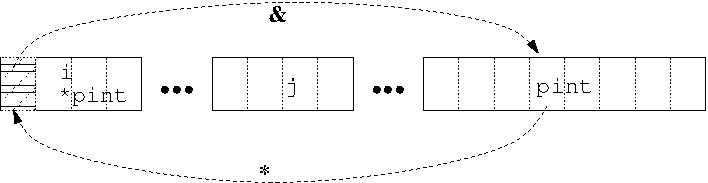
\includegraphics[scale=0.9]{kap621.pdf}}

\underline{Achtung :} In dem Programmfragment
\\[0.5ex]
\begin{minipage} {0.5\textwidth}
\begin{verbatim}
{
  double *px;
  *px = 3.1;     // WRONG!
}
\end{verbatim}
\end{minipage}
\\[0.5ex]
wird  zwar Speicherplatz  f"ur den Zeiger  reserviert  (8~Byte),
jedoch ist der  Wert von \verb|px| noch undefiniert und daher
wird der Wert \verb|3.1| in einen daf"ur nicht vorgesehenen
Speicherbereich geschrieben \\
$\Longrightarrow$ mysteri"ose Programmabst"urze und -fehler.
\index{Zeiger!undefiniert}

Es gibt eine spezielle Zeigerkonstante \verb| nullptr |
(\verb| NULL | in C), welche
auf die (hexadezimale) Speicheradresse \verb| 0x0 |
verweist und bzgl. welcher eine
Zeigervariable getestet werden kann.
\index{Zeiger!Nullpointer}
%
%
\subsection{Zeiger und Felder - Zeigerarithmetik}
\label{p:6.2.3}
%
Felder nutzen das Modell des linearen Speichers, d.h.,
ein im Index nachfolgendes Element ist auch physisch im
unmittelbar nachfolgenden Speicherbereich abgelegt.
Dieser Fakt erlaubt die Interpretation von  Zeigervariablen als
Feldbezeichner und umgekehrt.
\index{Zeiger!Arithmetik}

\begin{minipage} {0.9\textwidth}
\begin{verbatim}
{
  const int N = 10;
        int f[N], *pint;  // C-array and pointer

  pint = &f[0];           // init pointer
}
\end{verbatim}
\end{minipage}

Feldbezeichner werden prinzipiell als Zeiger behandelt, daher ist die
Programmzeile
\\
\mbox{}\hfill\verb| pint = &f[0]; |\hfill\mbox{}
\\
identisch mit
\\
\mbox{}\hfill\verb| pint = f; |\hfill\mbox{}
\\
Folgerichtig stellen daher die Ausdr"ucke
\verb| f[1] |, \verb| *(f+1) |, \verb| *(pint+1) |, \verb| pint[1] |
den identischen Zugriff auf das Feldelement $f_1$ dar.
\bspfile{Ex630.cpp}

% \input{kap631.pstex_t}
\centerline{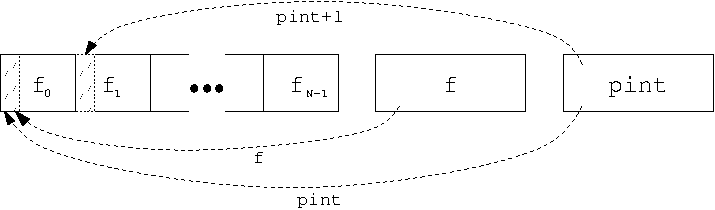
\includegraphics[scale=0.9]{kap631.pdf}}
%

Die Adresse welche durch (\verb|pint+1|) dargestellt wird
ergibt sich zu (Adresse in \verb|pint|) + \verb|sizeof(int) |.
Dabei bezeichnet \verb|int| den Datentyp, auf welchen der Zeiger
\verb|pint| verweist.
Der Zugriff auf andere Feldelemente $f_i$, $i=0\ldots N-1$ ist analog.

Die folgenden Operatoren sind auf Zeiger anwendbar:
\begin{itemize}
 \item Vergleichsoperatoren:
   \verb| == |, \verb| != |, \verb| < |, \verb| > |, \verb| <= |, \verb| >= |
 \item Addition \verb| + | und Subtraktion \verb| - |
 \item Inkrement \verb| ++ |, Dekrement \verb| -- |und
 	zusammengesetzte Operatoren \verb| += |, \verb| -= |
\end{itemize}

% \pagebreak
Zur Demonstration betrachten wir ein \textbf{Beispiel}, in welchem
ein Feld erst auf konventionelle Weise deklariert und initialisiert wird um
danach mittels Zeigeroperationen ausgegeben zu werden.
%\exfile{Ex630.cpp}

% \input{kap632.pstex_t}
\centerline{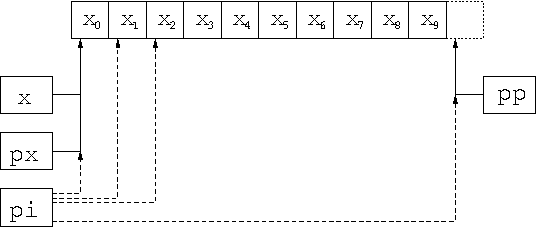
\includegraphics[scale=1.1]{kap632_b.pdf}}
%
%\includecode[linerange={9-15,19-19,23-23,26-27}]{Ex630.cpp}{Pointerarithmetik}
\includecode[firstline=6]{Ex630.cpp}{Pointerarithmetik}
%
In Listing~\ref{lst:Ex630.cpp} sind der Zählzyklus mit~\verb| i | als 
auch der Zählzyklus mit~\verb| pi | bzgl.\  der Zugriffe auf das C-Array~\verb| x | 
identisch. 

%%
%\begin{minipage} {0.9\textwidth}
%\begin{boxedverbatim}
%//	Pointers and arrays
%#include <iostream>
%main()
%{
  %const int N=10;
  %double    x[N], *px, *pp, *pi;
  %int       i;

%//                    initialize x
  %px = x;
  %for (i = 0; i < N; ++i )
   %{
     %*(px+i) = (i+1)*(i+1);    // x[i] = ...
   %}
%//              output x;
%//                       pointer pi as loop variable
  %pp = x+N-1;         // pointer at last element of x
  %for ( pi = x; pi <= pp; ++pi)
   %{
     %cout << "  " << *pi << endl;
   %}
%}
%\end{boxedverbatim}
%\end{minipage}

%
%


\section{Iteratoren}
\label{p:6.3}
Das Konzept der Zeiger, welches direkt an fortlaufende Adressen im Speicher gebunden ist, 
wird in C++ durch das Konzept der \emph{Iteratoren} erweitert. 
Dabei kann man sich die Iteratoren im einfachsten Fall von C++Feldern 
(\texttt{array}, \texttt{vector}) als Pointer vorstellen, 
jedoch spätestens bei Liste (\texttt{list}) muß man sich von dieser Simplifizierung lösen.
%
%
\subsection{Iteratorenzugriff auf \texttt{array}}
%
%
%\includecode[linerange={9-15,19-19,23-23,26-27}]{Ex630.cpp}{Pointerarithmetik}
\includecode[firstline=5]{bsp631a.cpp}{Iteratoren für C++-\texttt{array}}
%\verb|array|{}
%
Das obige Listing is analog zum Listing~\ref{lst:Ex630.cpp} für ein C-array. 
Auf folgende Unterscheide sei hingewiesen:
\begin{itemize}
	\item Zeile 8: Die Anfangsadresse der gespeicherten Daten ist nicht mehr \verb|&x|, sondern 
	   \verb|x.data()|. Der Ausdruck \verb|&x| liefert einen Pointer vom Typ \verb|array<double, 10>| zurück.
	\item Zeile 17: Die Laufvariable \verb|pi| ist jetzt ein Iterator, speziell für \verb|array<double, 10>|. 
	     Hätten wir ein zweites Array \verb|array<double, 33>|, dann könnte Iterator \verb|pi| nicht dafür 
	     verwendet werden (bei Pointern ginge dies.).
\end{itemize}

%In Zeilen



\section{Referenzen}
\label{p:6.1}
Referenzen sind ein Sprachmittel, um einen anderen Namen für dieselben Daten zu benutzen.
In Zeile~6 des Listings~\ref{lst:bsp611.cpp} wird eine Referenz~\texttt{ri} 
auf die Variable~\texttt{i} deklariert. Danach ist ein Zugriff auf~\texttt{ri} 
völlig äquivalent zu einem Zugriff auf~\texttt{i}.
%
\includecode[firstline=7]{bsp611.cpp}{Referenz}
%
Wozu benötigt man eigenlich Referenzen?
\begin{itemize}
	\item Um auf Teile aus einer größeren Struktur einfach zuzugreifen, 
	\emph{ohne diese kopieren} zu müssen. 
	\begin{verbatim}
	Student_Mult a;
	int &studium0 = a.skz[0];
	\end{verbatim}
	\item Als Kennzeichnung von Output-Parametern in der Parameterliste einer Funktion, siehe~\S\ref{p:7.3}.
	\item Mit vorgesetztem \texttt{const} zur Kennzeichnung von reinen Input-Parametern in der Parameterliste einer Funktion, siehe~\S\ref{p:7.3}. In diesem Falle werden die Daten nicht kopiert bei der Übergabe an die 
	Funktion. 
\end{itemize}


